\label{Appendix:TecplotUseage}
\section{\gwf\ Domain} \label{Tecplot:GWF}
To visualize the \gwf\ domain mesh:
\begin{enumerate}
    \item Start a command prompt in the folder which contains the \mut\ input file.
    \item Run \tecplot\ by typing:
        \begin{verbatim}
            tec360
        \end{verbatim}
    \item Choose 'Load Data' to open a file selection dialogue:

        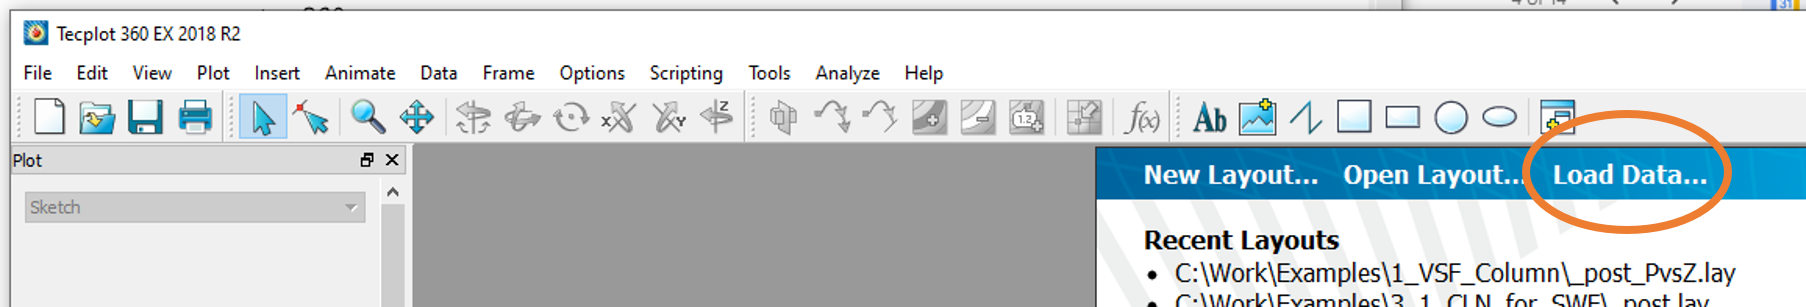
\includegraphics[width=\textwidth]{Tecplot_1_GWF}

    \item Select and open the file \texttt{\_buildo.Modflow.GWF.tecplot.dat}:

        \includegraphics[width=\textwidth]{Tecplot_2_GWFfiles}

   \item Click the 'Mesh' checkbox, then choose 'Yes' to turn on surfaces for active zones.

        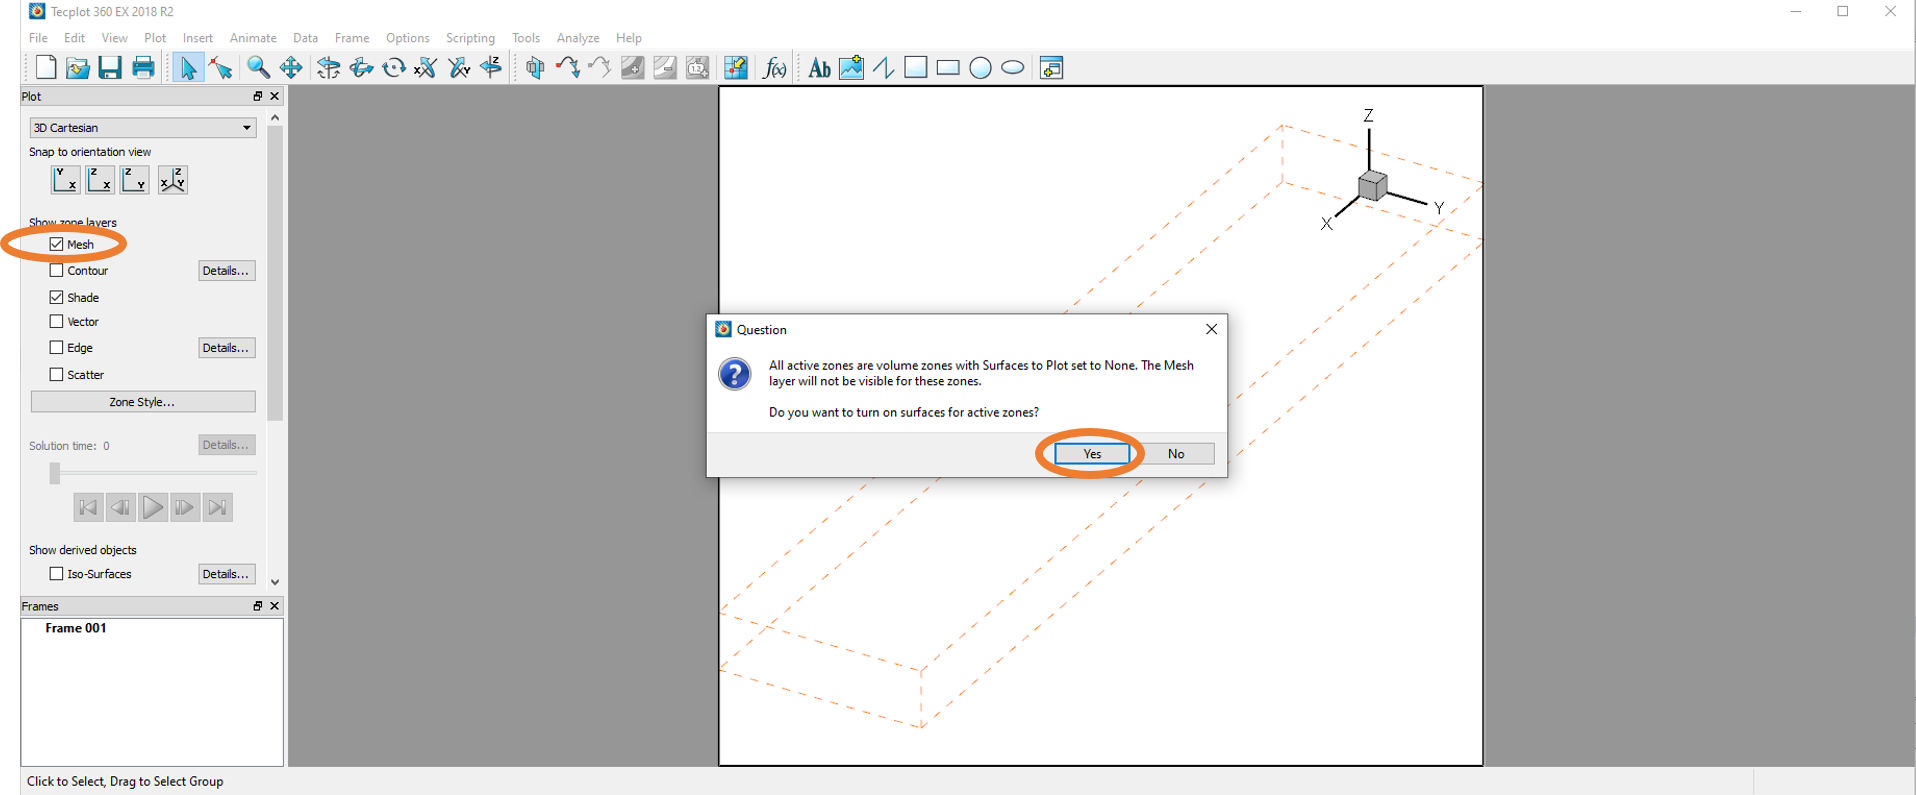
\includegraphics[width=\textwidth]{Tecplot_3_GWFMesh}

\end{enumerate}
You will now see the finite-element mesh that was used to define the \mfus\ \gwf\ domain cells:

        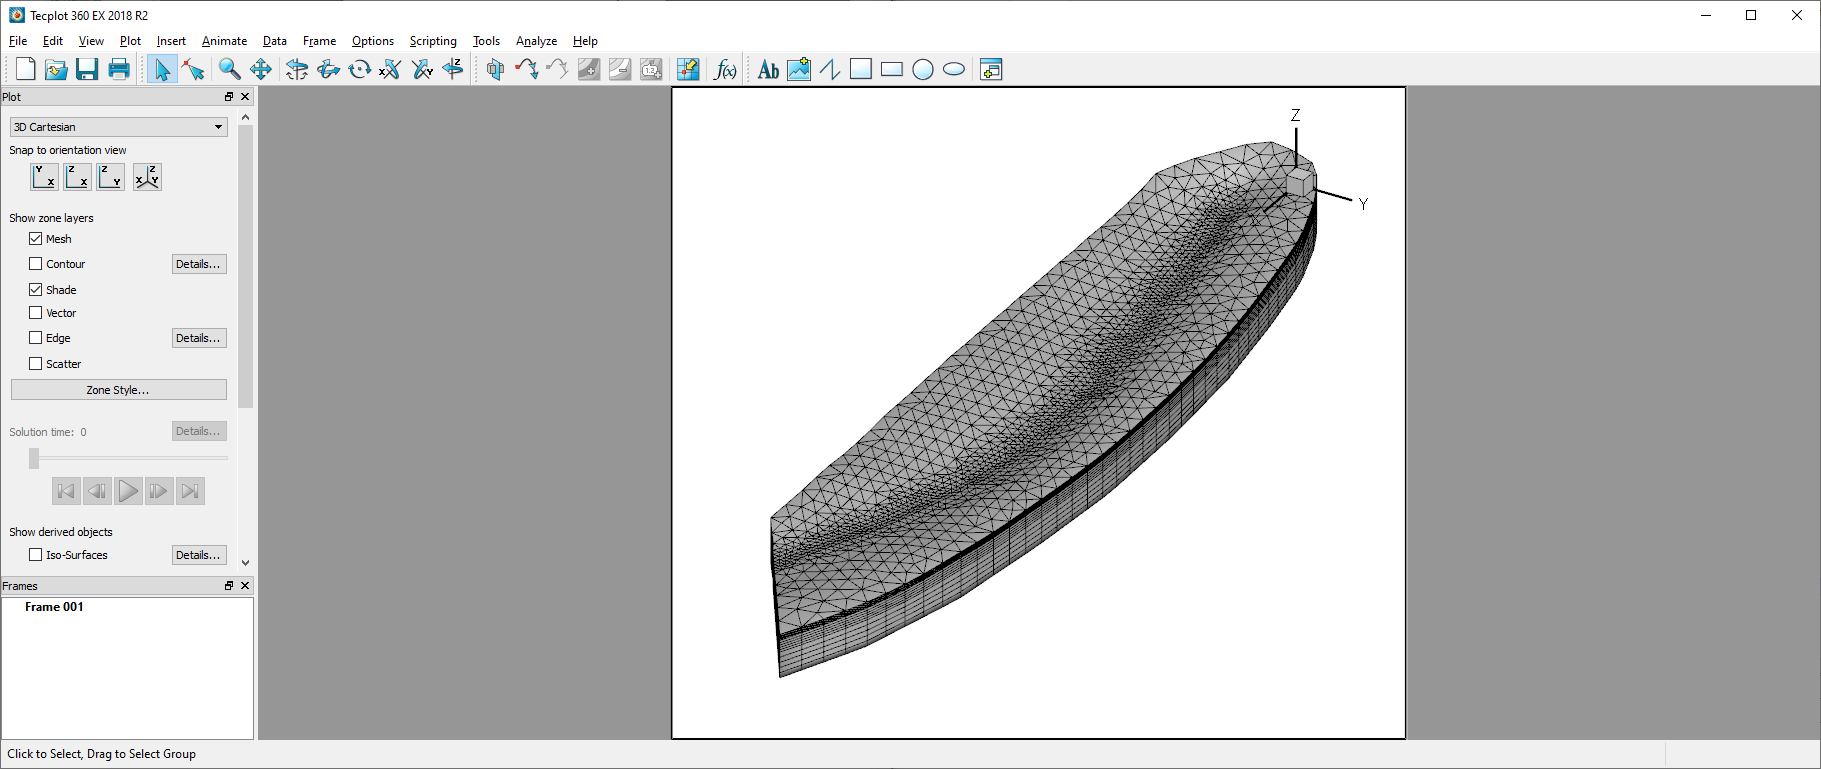
\includegraphics[width=.8\textwidth]{Tecplot_4_GWFMesh}

\section{Using the Probe Tool} \label{Tecplot:ProbeTool}
Select the Probe At Tool 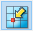
\includegraphics{ProbeToolButton} to probe for values of the dataset's variables at a particular point.

The mouse cursor changes to a modified cross-hair which indicates the Probe Tool is active.

To obtain interpolated values of the dataset variables at the specified location, click at any point in the data region.

To obtain exact values for the data point nearest the specified location, Control-click at the desired location.

For XY plots, when you move into the axis grid area, the cursor cross hair is augmented by a vertical or horizontal line, depending on whether you are probing along the X-axis or the Y-axis. You can change the axis to probe simply by pressing X to probe the X-axis or Y to probe the Y-axis.




%\section*{Step~\ref{step:Tecplot1}: Run \tecplot\ to Examine the Built Project}
%You can run \tecplot\ and load the \tecplot\ layout file \_\verb+build.lay+ by typing:
%\begin{verbatim}
%    tec360 _build.lay
%\end{verbatim}
%Some key features to note are:
%\begin{itemize}
%    \item A \tecplot\ window should open: \\ \\
%        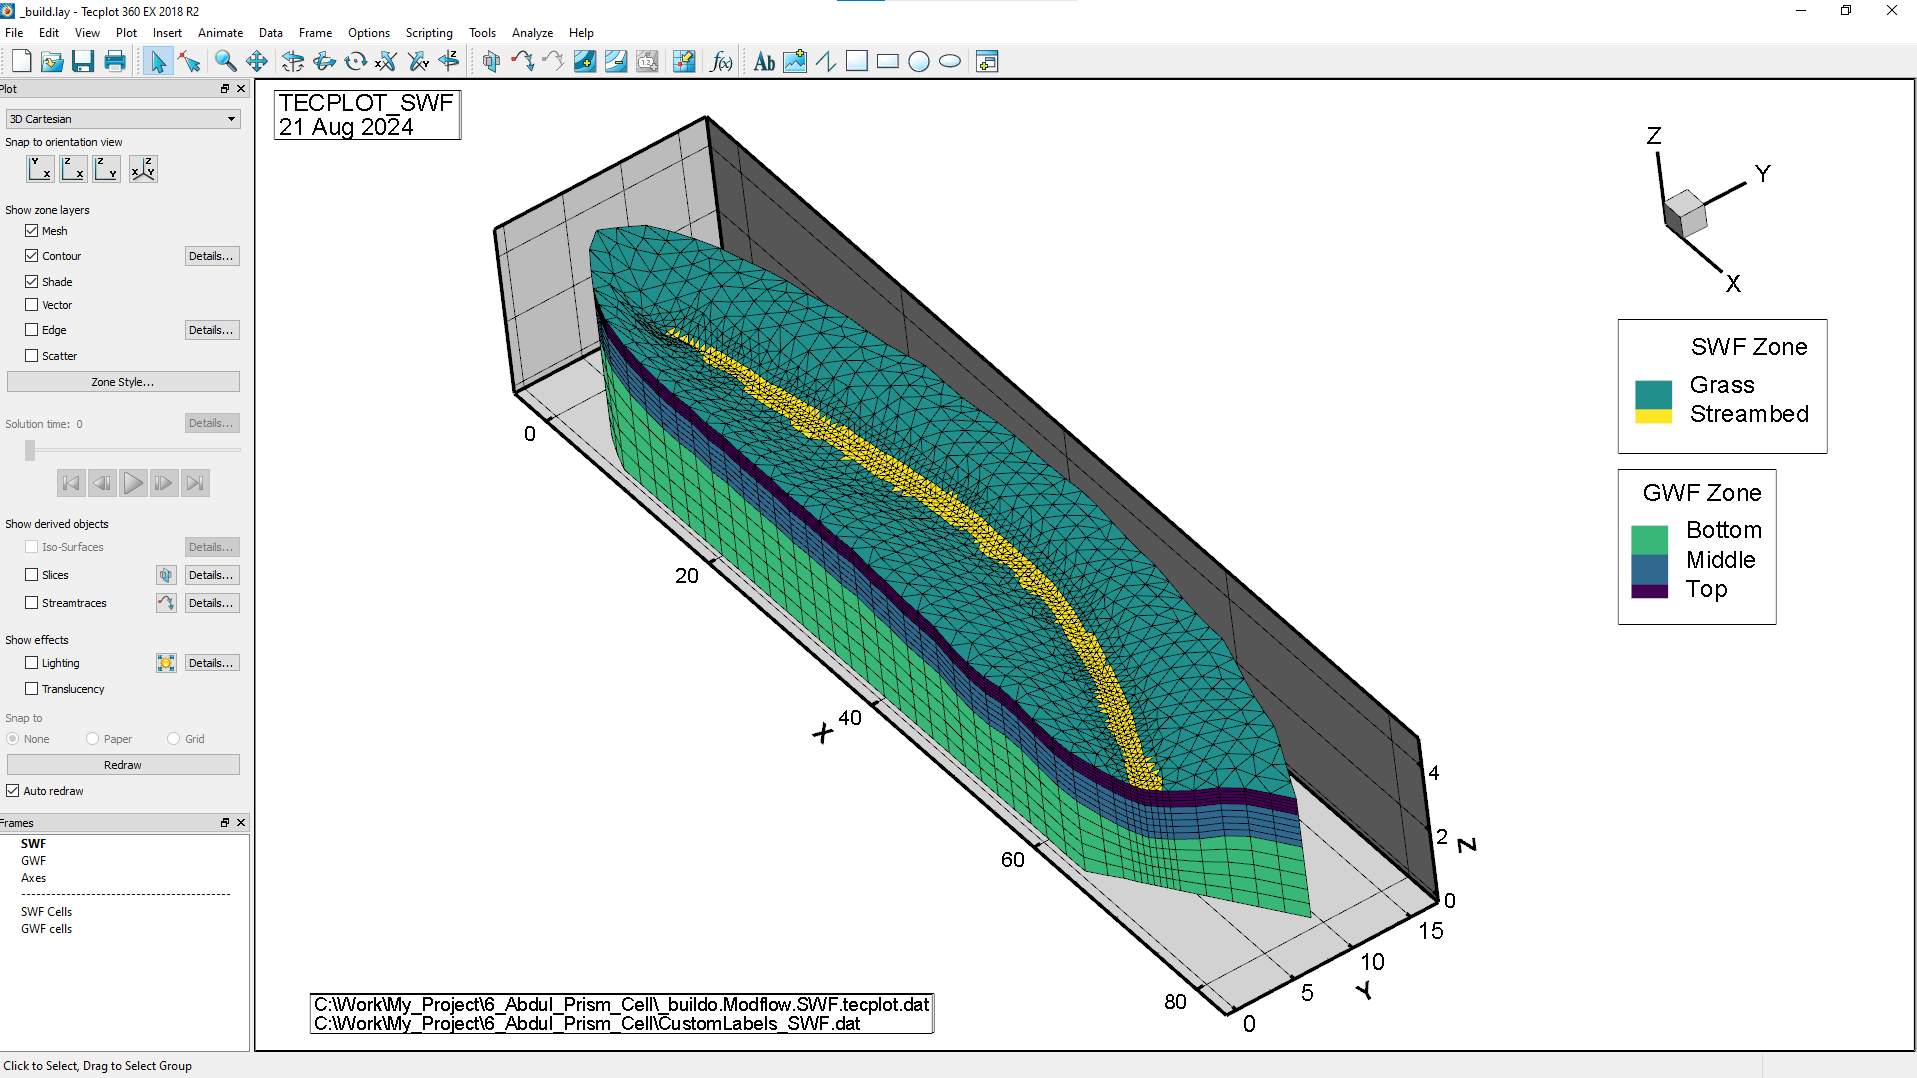
\includegraphics[width=0.8\textwidth]{TecplotBuild} \\ \\
%    This \tecplot\ layout file has been constructed with multiple frames (see lower left 'Frames' window) showing details about the\swf\ and\gwf\ model domains. This default view shows the distribution of the various materials defined in the model, such as the\swf\ domain materials called 'Grass' and 'Streambed'.  Detailed information about manipulating the data in \tecplot\ to produce the desired plots is discussed in Section~\ref{Tecplot}.
%    \item \tecplot\ data can be probed using the probe tool 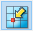
\includegraphics{ProbeToolButton} .  Here we see the results of probing a location in the\swf\ domain: \\
%        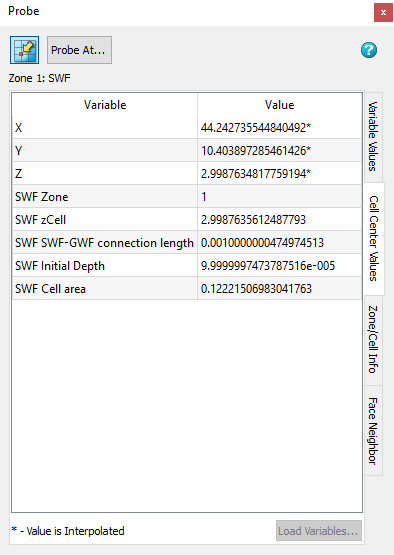
\includegraphics[width=0.4\textwidth]{SWFprobe} \\
%       \swf\ results were returned because the\swf\ frame is at the front of the frame stack.
%    \item In order to probe the\gwf\ domain we have to move it to the front of the stack: \\
%            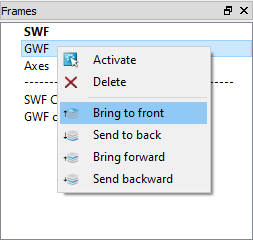
\includegraphics[width=0.4\textwidth]{BringToFront} \\
%          Here we see the results of probing a location in the\gwf\ domain: \\
%            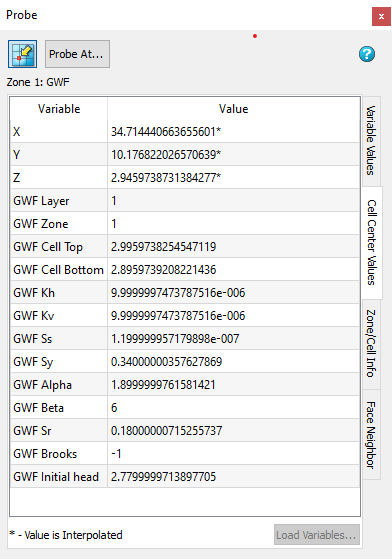
\includegraphics[width=0.4\textwidth]{GWFprobe} \\
%
%\end{itemize}
%
